\documentclass{article}

\usepackage{graphicx}
\usepackage{color}

\begin{document}

\title{jStar Eclipse tutorial} 
\maketitle 


\section{Installation}

Two ways:
\begin{enumerate}
\item Add the jar file com.jstar.eclipse\_1.0.0.jar to \texttt{eclipse/dropins/} folder and restart Eclipse.
\item {\color{red} Need to create update site.}
\end{enumerate}

\section{Configuration}

On Windows with cygwin:

Go to Windows $\rightarrow$ Preferences $\rightarrow$ jStar Configuration and set the required directories.\\

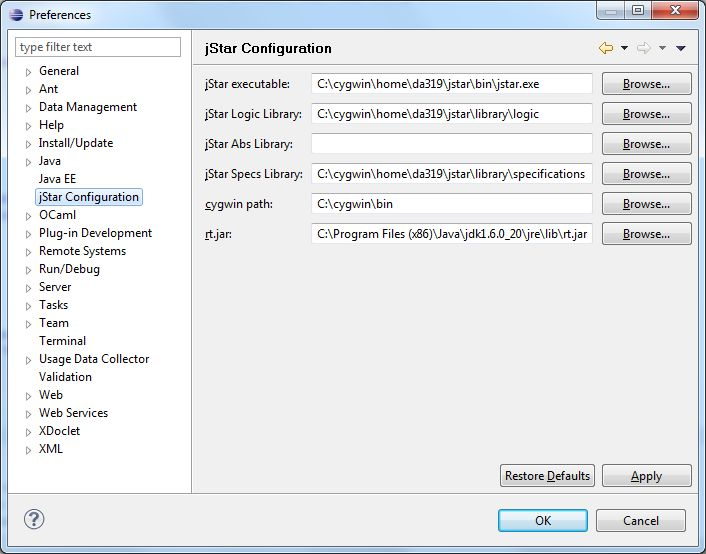
\includegraphics[width=4in]{images/preferences.jpg}

\section{Verification}
Press right mouse button to open context menu and select \texttt{Verify with jStar...}.
In the pop-up window indicate the location of specification, logic and abstraction rules.\\

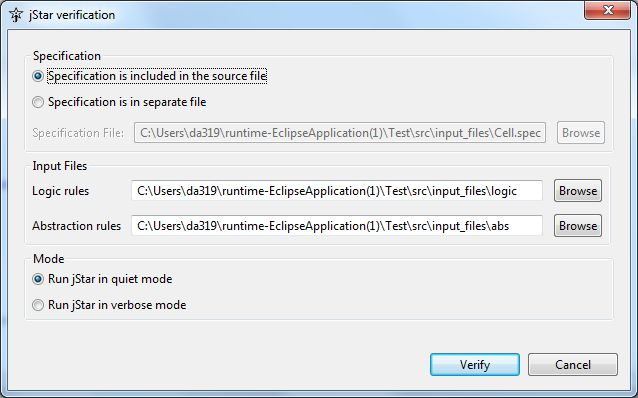
\includegraphics[width=4in]{images/verificationWindow.jpg}
\\\\Click Verify. 

\subsection* {Verification errors}

In case there are some verification errors, one can see error messages in console and lines in source code where the problem appeared are annotated as squiggly marks.\\

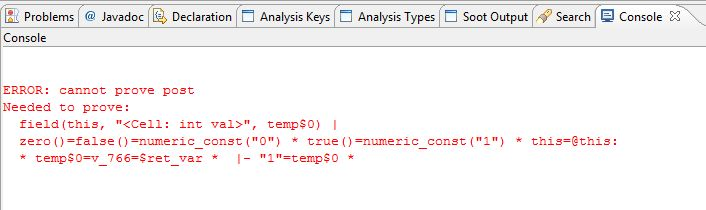
\includegraphics[width=4in]{images/console.jpg}\\

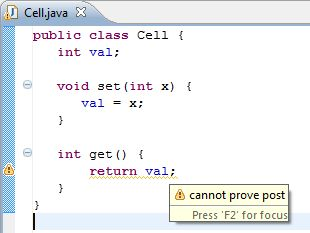
\includegraphics[width=2in]{images/marker.jpg}



\end{document}